\documentclass[12pt]{article}
\usepackage{amsmath, amssymb, amsthm}
\usepackage{import}
\usepackage{pdfpages}
\usepackage{transparent}
\usepackage{xcolor}
\usepackage{graphicx}

\usepackage{fancyhdr}

\fancyhf{}
\pagestyle{fancy}
\lhead{Carrera}
\rhead{\thepage}

\setlength\parindent{0pt}
\numberwithin{equation}{section}

\usepackage{titlesec}
\titleformat{\section}
{\normalfont\Large\bfseries}{Exercise~\thesection}{1em}{}

\newcommand{\incfig}[2][1]{%
  \def\svgwidth{#1\columnwidth}
  \import{./figures/}{#2.pdf_tex}
}

\newcommand{\RE}{\mathrm{Re}}
\newcommand{\IM}{\mathrm{Im}}

\newcommand\ddfrac[2]{\frac{\displaystyle #1}{\displaystyle #2}}

\pdfsuppresswarningpagegroup=1

\author{Adam Carrera}
\date{January 30, 2021}
\title{MECH 3340 - Assignment \#1}

\begin{document}
  \maketitle
  \section{}
  Given,
  \[
      z = \frac{-1 + j\sqrt{3}}{\sqrt{3} + j}
    .\]

  Multiply $ z $ by 1 and simplify.

  \begin{equation}
    \frac{-1 + j\sqrt{3}}{\sqrt{3} + j} \left( \frac{\sqrt{3} - 1}{\sqrt{3} - 1} \right) = \frac{-\sqrt{3} -j^2 \sqrt{3} + j + 3j}{4}
  \end{equation}

  \begin{equation}
    \frac{-\sqrt{3} + \sqrt{3} + 4j}{4} = j \Rightarrow \RE(z) = 0, \quad \IM(z) = j
  \end{equation}

  Magnitude and Phase,

  \begin{equation}
    r = \sqrt{\RE(z)^2 + \IM(z)^2} = \sqrt{1^2} = 1
  \end{equation}

  \begin{equation}
    \theta = \tan^{-1} \left( \frac{\RE(z)}{\IM(z)} \right) = \tan^{-1} \left( \frac{0}{1} \right) = \frac{\pi}{2}
  \end{equation}

  \newpage
  \section{}
  Given,
  \[
      \bar{z} = \frac{5}{(2+j)}
    .\]

  Mutiply $ z $ by $ -1. $

  \begin{equation}
    \frac{5}{(2+j)} \left( \frac{2 - j}{2 - j} \right) = \frac{10 - j5}{3}
  \end{equation}

  This implies that,

  \begin{equation}
    z = \frac{10 + j5}{3}
  \end{equation}

  However, $ \theta $ lies in the second quadrant.
  \begin{equation}
    \theta = \tan^{-1} \left( \frac{10/3}{5/3} \right) = \tan^{-1}(2)
  \end{equation}

  Therefore, a complex number with conjugate $ \bar{z} $ cannot exist in the fourth quadrant.

  \section{}

  Factor $ z^3 + 27 = 0 $ as a sum of two cubes.

  \begin{equation}
    z^3 + 27 = (z + 3)(z ^2 - 3z + 9)
  \end{equation}

  Clearly, $ z_1 = -3. $ The other two roots can be found with the quadratic formula.

  \begin{equation}
    z_2, z_3 = \frac{3 \pm \sqrt{9 - 36}}{2} = \frac{3}{2} \pm j \frac{\sqrt{27}}{2}
  \end{equation}

  \newpage

  $ z_1, z_2, z_3 $ are in rectangular form. In polar form,

  \begin{align}
    r_1 &= \sqrt{(-3)^2} = -3, \quad \theta_1 = \tan^{-1} \left( \frac{0}{3} \right) = 0 \\
    r_2 &= \sqrt{ \left( \frac{3}{2} \right)^2 + \left( \frac{\sqrt{27}}{2} \right)^2 } = 3, \quad \theta_2 = \tan^{-1} \left( \frac{\sqrt{27}/2}{3/2} \right) = 60^{\circ} \\
    r_3 &= 3, \quad \theta_3 = -60^{\circ}
  \end{align}

  Therefore,

  \begin{align}
    z_1 &= -3e^{j \cdot 0} = -3 \\
    z_2 &= 3e^{j \frac{\pi}{3}} \\
    z_3 &= 3e^{-j \frac{\pi}{3}}
  \end{align}

  \newpage

  \section{}
  Given that,

  \[
      G(j) = \frac{j - 1}{j + \sqrt{2}}
    .\]

  The magnitude and phase of $ G(j) $ are 0.8165 and 1.7407, respectively. Figure \ref{fig:fig1} shows the matlab commands used and their output.

  \begin{figure}
    \centering
    \normalsize
    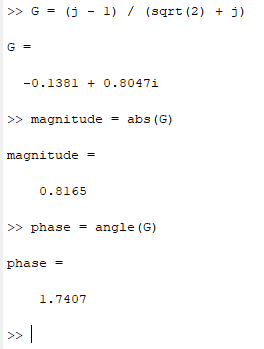
\includegraphics{./figures/fig1}
    \caption{MATLAB Commands for Exercise 4}
    \label{fig:fig1}
  \end{figure}

  \newpage

  \section{}

  \subsection{$\sin(A+B) = \sin A \cos B$}

  \begin{proof}
    Let $ \theta = A + B. $ Using euler's formula, we know that

    \begin{equation} \label{eqn:eq1}
      \sin \theta = \ddfrac{e^{j \theta} - e^{-j \theta}}{2j}
    \end{equation}

    Substitute $ \theta = A + B$ into Equation (\ref{eqn:eq1}).

    \begin{equation} \label{eqn:eq2}
      \sin(A+B) = \ddfrac{e^{jA}e^{jB} - e^{-jA}e^{-jB}}{2}
    \end{equation}

    Substitute $ e^{j \theta} = \cos \theta + j\sin \theta $ into the RHS  of Equation (\ref{eqn:eq2}) and simplify.

    \begin{equation}
      \frac{(\cos A + j\sin A)(\cos B + j\sin B) - (\cos A - j\sin A)(\cos B - j\sin B)}{2j}
    \end{equation}

    \begin{equation}
      \sin(A+B) = \frac{2j \cos A \sin B + \sin A \cos B}{2j}
    \end{equation}

    \begin{equation}
      \sin(A+B) = \cos A \sin B + \sin A \cos B \tag*{\qedhere}
    \end{equation}
  \end{proof}

  \subsection{$\cos 2\theta = 1 - 2\sin^2 \theta$}

  \begin{proof}
    Let $ \theta = A = B. $ We know that,

    \begin{equation}
      2\cos \theta = e^{j\theta} + e^{-j\theta}
    \end{equation}

    Substitute $ \theta = A + B. $

    \begin{equation}
      2\cos(A + B) = e^{jA}e^{jB} + e^{-jA}e^{-jB}
    \end{equation}

    $ \theta = A = B $ implies that,

    \begin{equation}
      2\cos 2\theta = e^{j\theta}e^{j\theta} + e^{-j\theta}e^{-j\theta}
    \end{equation}

    \newpage

    Examine the RHS and expand the two squared terms.

    \begin{equation}
      =(\cos\theta + j\sin\theta)^2 + (\cos\theta - j\sin\theta)^2
    \end{equation}

    \begin{equation}
      =(\cos^2\theta + 2j\sin\theta\cos\theta - \sin^2\theta) + (\cos^2\theta - 2j\sin\theta\cos\theta - \sin^2\theta)
    \end{equation}

    \begin{equation}
      \cos2\theta = \cos^2\theta - \sin^2\theta
    \end{equation}

    Using identity $ \sin^2 + \cos^2 = 1. $

    \begin{equation}
      \cos2\theta = 1 - \sin^2\theta - \sin^2\theta
    \end{equation}

    \begin{equation}
      \cos2\theta = 1 - 2\sin^2\theta \tag*{\qedhere}
    \end{equation}
  \end{proof}

  \section{}

  \begin{itemize}
    \item $\dot x + x -e^x = 0$ is 1st order, nonlinear, and homogeneous
    \item $\ddot x + t\dot x + x = 0$ is 2nd order, linear, and homogeneous
    \item $\dddot x + \dot x + x ^2 - \cos t = 0$ is 3rd order, nonlinear, and homogeneous
  \end{itemize}

  \newpage

  \section{}

  Given,

  \[
      \dot x + x = 2 e^{-t}, \quad x(0^{-}) = -1
    .\]

  \subsection{Homogeneous Solution}

  The homogeneous equation is given by

  \begin{equation} \label{eqn:eq3}
    \dot x + x = 0
  \end{equation}

  Substitute $ x(t) = e^{\lambda t} $ into Equation (\ref{eqn:eq3}).

  \begin{align}
    \lambda e^{\lambda t} + e^{\lambda t} &= 0 \\
    e^{\lambda t} (1 + \lambda) = 0
  \end{align}

  Clearly, $ \lambda = -1. $ Using ICs we can find the value of $ C. $

  \begin{align}
    x(t) &= Ce^{-t} \\
    -1 &= Ce^0 \\
    C &= -1
  \end{align}

  Therefore, $ x_h = -e^{-t}. $

  \newpage

  \subsection{Particular Solution}
  The form of the particular solution cannot be proportional to the form of the homogeneous solution.
  \[
      f(t) = 2e^{-t} \Rightarrow x_p(t) = Cte^{-t}
    .\]

  Substitute $ x_p $ into the original differential equation.
    \begin{align}
      C \left( e^{-t} -te^{-t} \right) + Ct e^{-t} &= 2e^{-t} \\
      Ce^{-t} &= 2e^{-t} \\
      C &= -2 \Rightarrow x_p(t) = 2te^{-t}
    \end{align}

  The total response is the sum of the particular and homogeneous solutions.

  \begin{equation}
    x = 2te^{-t} - e^{-t}
  \end{equation}

  \section{}

  Find the family of solutions for,

  \[
      \ddot x + 2 \dot x + x = \sin2t
    .\]

  \subsection{Homogeneous Solution}

  The characteristic equation is given by,

  \begin{align}
    \left( \lambda ^2 + 2 \lambda + 1 \right) &= 0 \\
    (\lambda + 1) ^2 &= 0
  \end{align}

  \[
      \lambda = -1, 1
    .\]

  This implies that,

  \begin{equation}
    x_h(t) = C_1 e^{-t} + C_2 te^{-t}
  \end{equation}

  \subsection{Particular Solution}

  \[
      f(t) = \sin2t \Rightarrow x_p = C\sin2t
    .\]

  Substitute $ x_p. $

  \begin{align}
    -4C\sin2t + 4C\cos2t +c\sin2t &= \sin2t \\
    C \left( \sin2t - 4\sin2t + 4\cos2t \right) &= \sin2t \\
    C \left( -3\sin2t + 4\cos2t \right) &= \sin2t \\
  \end{align}

  \begin{equation}
      C = \ddfrac{\sin2t}{-3\sin2t + 4\cos2t}
  \end{equation}
  Therefore,
  \begin{equation}
    x_p = \ddfrac{\sin^22t}{-3\sin2t + 4\cos2t}
  \end{equation}

  \begin{equation}
    x(t) = C_1 e^{-t} + C_2 te^{-t} + \ddfrac{\sin^22t}{-3\sin2t + 4\cos2t}
  \end{equation}






  \section{}

  Given two coupled ODEs,

  \begin{align}
    3\dot x_1 + 5 x_1 - 7x_2 &= 5 \label{eqn:eq4}\\
    \dot x_2 + 4x_1 + 6x_2 &= 0 \label{eqn:eq5}
  \end{align}

  Take the derivative of Equation (\ref{eqn:eq4}).

  \begin{equation}
    3\ddot x_1 + 5\dot x_1 - 7 x_2 = 0
  \end{equation}

  \begin{equation} \label{eqn:eq6}
    \dot x_2 = \frac{3}{7} \ddot x_1 + \frac{5}{7} \dot x_1
  \end{equation}

  We can use Equation (\ref{eqn:eq6}) to rewrite Equations (\ref{eqn:eq4}) and (\ref{eqn:eq5}) as one ODE.
  \begin{equation}
    \frac{3}{7}\ddot x_1 + \frac{5}{7} \dot x_1 + 4 x_1 + 6 x_2 = 0
  \end{equation}



\end{document}
